\documentclass{standalone}
\usepackage{tikz}
\usepackage{ctex,siunitx}
\usepackage{tkz-euclide}
\usepackage{amsmath}
\usetikzlibrary{patterns, calc}
\usetikzlibrary {decorations.pathmorphing, decorations.pathreplacing, decorations.shapes,3d}
\tikzset{
pencil/.pic={
  \fill[left color =green!80!black,right color=green!80!black,middle color=white](-0.05,0.2)rectangle(0.05,1.5);
  \fill[left color =brown,right color=brown,middle color=white](-0.05,0.2)--(0,0)--(0.05,0.2);
  \fill(-0.02,0.08)--(0,0)--(0.02,0.08);
}
}
\begin{document}
\small
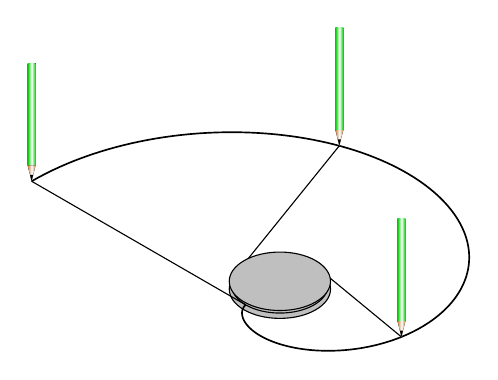
\begin{tikzpicture}[z={(-30:10mm)},x={(-150:10mm)},>=latex,scale=0.5,inner sep=1pt]
  \begin{scope}[canvas is xz plane at y=-0.1]
    \draw[fill=lightgray](0,0)circle(1.05);
  \end{scope}
  \begin{scope}[canvas is xz plane at y=0]
  \draw(0,0)circle(1);
  \draw[semithick,domain=0:360,samples=200] plot ({cos(\x)+\x/180*pi*sin(\x)},{sin(\x)-\x/180*pi*cos(\x)});
  \foreach \x in {170,290,360}
  {
    \draw(\x:1)--({cos(\x)+\x/180*pi*sin(\x)},{sin(\x)-\x/180*pi*cos(\x)}) pic {pencil};
  }
  \end{scope}
  \begin{scope}[canvas is xz plane at y=0.1]
    \draw[fill=lightgray](0,0)circle(1.05);
  \end{scope}
  % \foreach \x in {170,290,360}
  % {
  %   \draw({cos(\x)+\x/180*pi*sin(\x)},0,{sin(\x)-\x/180*pi*cos(\x)})--++(0.1,0.3,0)--++(0,1,0)--++(-0.2,0,0)--++(0,-1,0)--cycle;
  % }
\end{tikzpicture}
\end{document}